\newpage
\section{Komponenten}\label{sec:komponenten}
Für den Aufbau des Versuchs werden verschiedene Komponenten verwendet.
Diese werden im folgenden Kapitel vorgestellt.

\begin{description}
    \item[Sony Playstation 4 \cite{PS4Welco38:online}]
        Die \ac{ps4} ist eine Spielekonsole der aktuellsten Generation.
        Zusätzlich zur Funktion Spiele zu spielen, bietet die \ac{ps4}
        unter anderem auch die Möglichkeit Entertainment-Apps zu nutzen, um zum Beispiel Blue-Rays anzuschauen
        oder Streamingdienste wie \textit{Amazon Instant Video} oder \textit{Netflix} zu nutzen.

        \begin{figure}[h!]
            \centering
            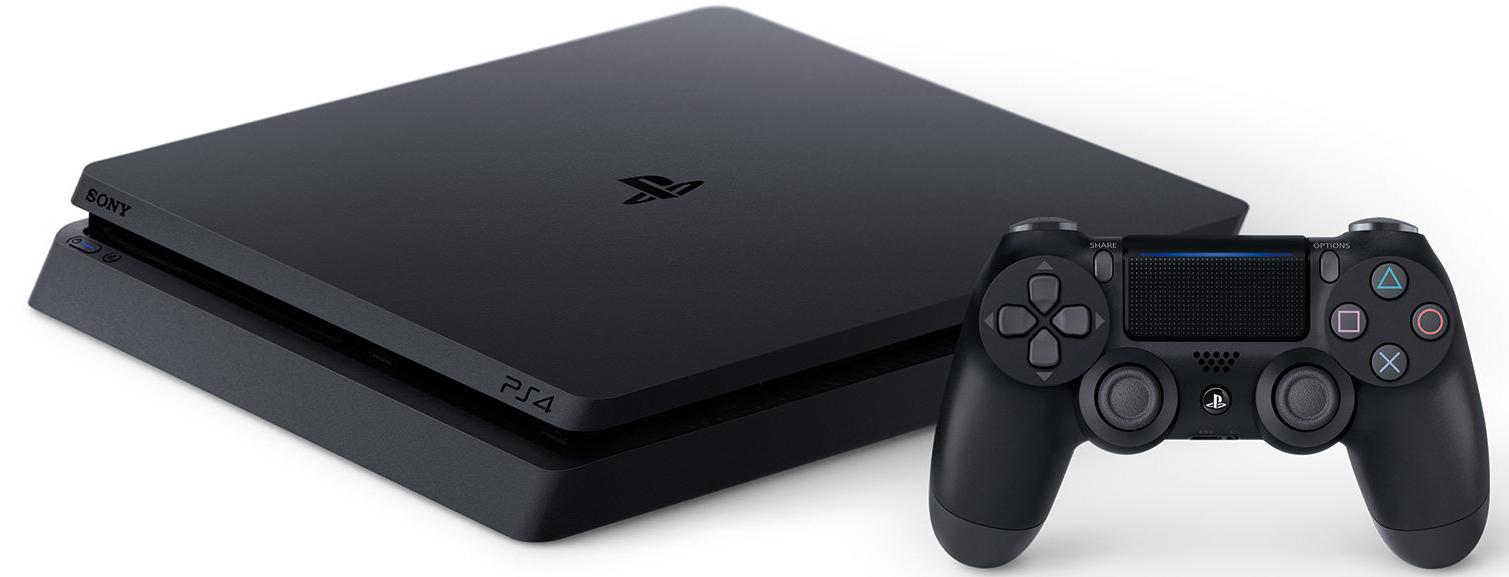
\includegraphics[width=0.5\textwidth]{ps4}
            \caption{Playstation 4 mit Controller}\label{fig:ps4}
        \end{figure}

        Gesteuert wird die Konsole in der Regel, durch einen Controller, welcher hauptsächlich für Spiele konzipiert wurde.
        Alternativ können auch diverse Bluetooth-Geräte oder eine Smartphone-App genutzt werden.

    \item[Raspberry Pi \cite{Whatisth47:online}]
        Der Raspberry Pi ist ein Einplatinencomputer \cite{Einplati37:online}, also ein Computer,
        bei welchem sich alle benötigten Komponenten auf einer einzigen Leiterplatte befinden.
        In diesem Projekt wird das Modell \textit{Raspberry Pi 3 Model B} verwendet.
        Hierzu zählen beim Raspberry Pi unter anderem die CPU, ein HDMI-Anschluss, mehrere USB-Buchsen sowie ein LAN-Anschluss.
        Betrieben wird er über ein Betriebssystem, welches auf einer Micro-SD installiert wird.

        \begin{figure}[h!]
            \centering
            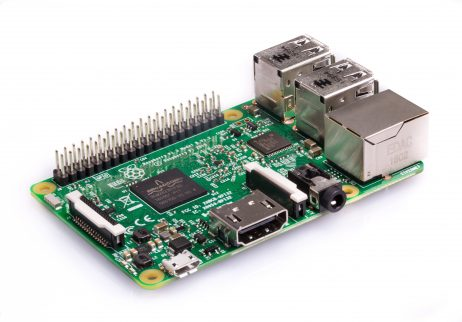
\includegraphics[width=0.5\textwidth]{pi}
            \caption{Raspberry Pi 3 Model B \cite{Raspberr2:online}}\label{fig:pi}
        \end{figure}

        Das offiziell unterstütze Betriebssystem ist \textit{Raspbian}, welches auf dem Linux-Betriebssystem \textit{Debian} basiert.
        Mit diesem Betriebssystem bietet der Raspberry Pi nahezu alle Möglichkeiten, welche auch ein klassischer Computer bietet.
        Eine Einschränkung ist jedoch, dass der Pi lediglich einen ARM-Prozessor besitzt.
        Programme, welche nur für x86- oder x64-Prozessoren entwickelt wurden, können somit nicht ausgeführt werden.

        Anstelle von \textit{Raspbian} können auch andere Betriebssysteme installiert werden,
        welche besser auf einen bestimmten Anwendungsfall zugeschnitten sind.

    \item[Home Assistant \cite{HomeAssi51:online}]
        Home Assistant ist eine open-source Plattform zur Heimautomatisierung.
        Basierend auf der Programmiersprache \textit{Python 3} ist sie gedacht,
        um auf einem Raspberry Pi ausgeführt zu werden.
        Mit \textit{Hassbian} wird ein Betriebssystem basierend auf \textit{Raspbian} angeboten,
        auf welchen Home Assistant bereits installiert und grundlegend konfiguriert ist.

        \begin{figure}[h!]
            \centering
            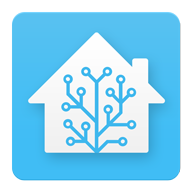
\includegraphics[width=0.25\textwidth]{homeassistant}
            \caption{Logo Homeassistant}\label{fig:homeassistant}
        \end{figure}

        Die Plattform ermöglicht das Überwachen und Steuern verschiedener Geräte zu Heimautomatisierung.
        Für dieses Projekt wird sie so konfiguriert,
        dass sie den Status der Playstation 4 überwacht und das Ein- sowie Ausschalten ermöglicht.
        Details zu dieser Konfiguration finden sich in Kapitel \ref{sec:aufbau} \textit{\nameref{sec:aufbau}}.

    \item[Logitech Harmony \cite{HarmonyH15:online}]
        Logitech Harmony ist die Fernbedienungs-Sparte von Logitech.
        In diesem Projekt wird der Harmony Hub zusammen mit der zugehörigen Harmony Elite Fernbedienung verwendet,
        Durch den Harmony Hub könne zahlreiche Geräte über Infrarot, WLAN oder Bluetooth gesteuert werden.
        Die Fernbedienung selbst kommuniziert hierbei über Funk \cite{HowToPoi90:online} mit dem Hub.
        Der Hub gibt die Befehle dann an die entsprechenden Geräte weiter.
        Zusätzlich lässt sich der Hub über eine Smartphone-App ansteuern.

        \begin{figure}[h!]
            \centering
            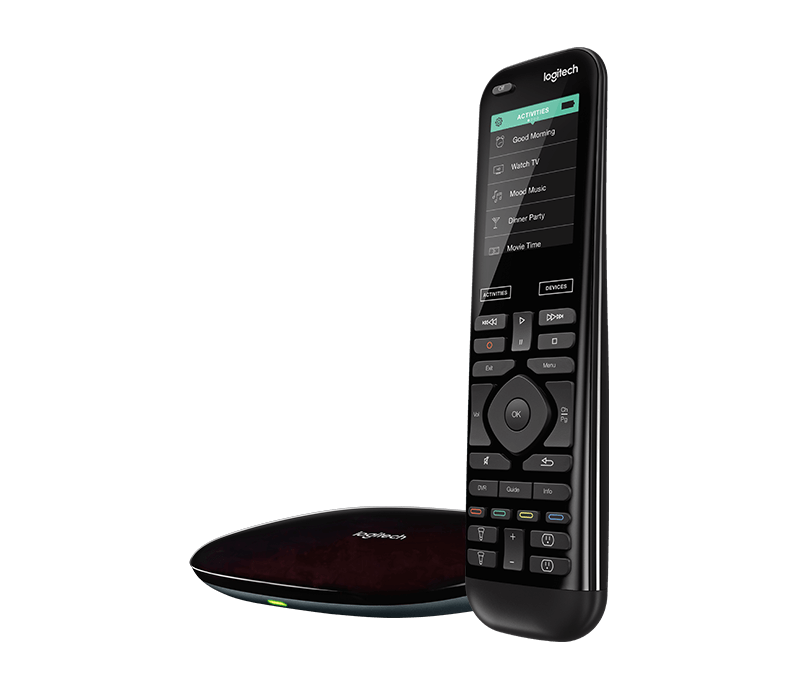
\includegraphics[width=0.5\textwidth]{harmony-elite}
            \caption{Hub, Fernbedienung und Smartphone mit App}\label{fig:harmony}
        \end{figure}

        Neben den verschiedenen Verbindungsmöglichkeiten ist ein großer Vorteil das Konfigurieren von \enquote{Aktionen}.
        Diese Stellen eine Sammlung von Befehlen an verschiedene Geräte dar.
        So kann beispielsweise über einen Tastendruck gleichzeitig Fernseher und Receiver eingeschaltet
        und (entsprechende Smart-Home-Geräte vorausgesetzt) das Licht gedimmt werden.
\end{description}